%%%%%%%%%%%%%%%%%%%%%%%%%%%%%%%%%%%%%%
%%%%%%%%%%%%%%%%%%%%%%%%%%%%%%%%%%%%%%
% Do not edit the TeX file your work
% will be overwritten.  Edit the RnW
% file instead.
%%%%%%%%%%%%%%%%%%%%%%%%%%%%%%%%%%%%%%
%%%%%%%%%%%%%%%%%%%%%%%%%%%%%%%%%%%%%%



\newcommand{\SimPathologicalRTwoFig}{

\begin{knitrout}
\definecolor{shadecolor}{rgb}{0.969, 0.969, 0.969}\color{fgcolor}\begin{figure}[!h]

{\centering 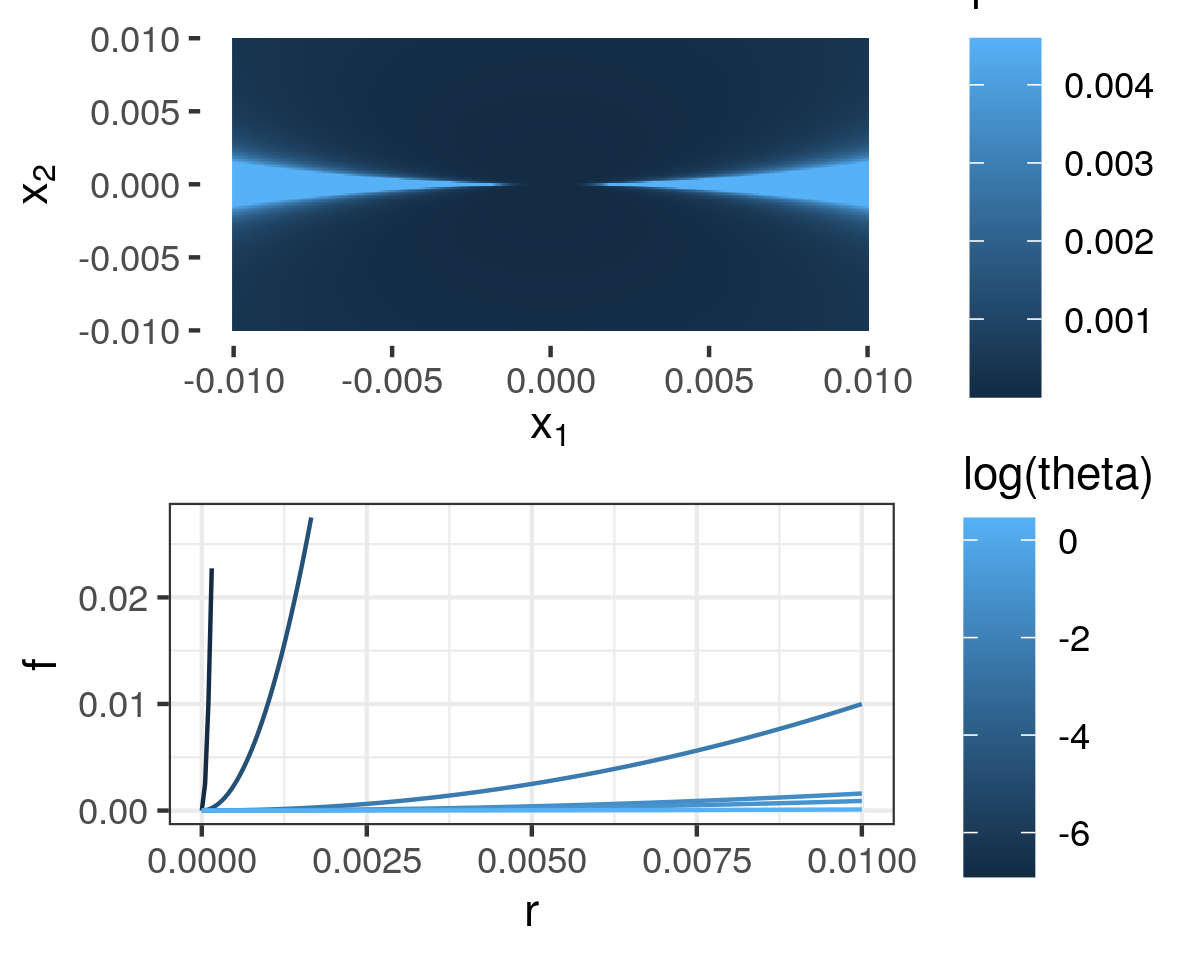
\includegraphics[width=0.980\linewidth,height=0.784\linewidth]{figure/r2_pathological-1} 

}

\caption[A plot of $f(x_1, x_2)$ from \exref{r2_pathological}]{A plot of $f(x_1, x_2)$ from \exref{r2_pathological}.}\label{fig:r2_pathological}
\end{figure}


\end{knitrout}
}


\newcommand{\SimPositivePertFig}{

\begin{knitrout}
\definecolor{shadecolor}{rgb}{0.969, 0.969, 0.969}\color{fgcolor}\begin{figure}[!h]

{\centering 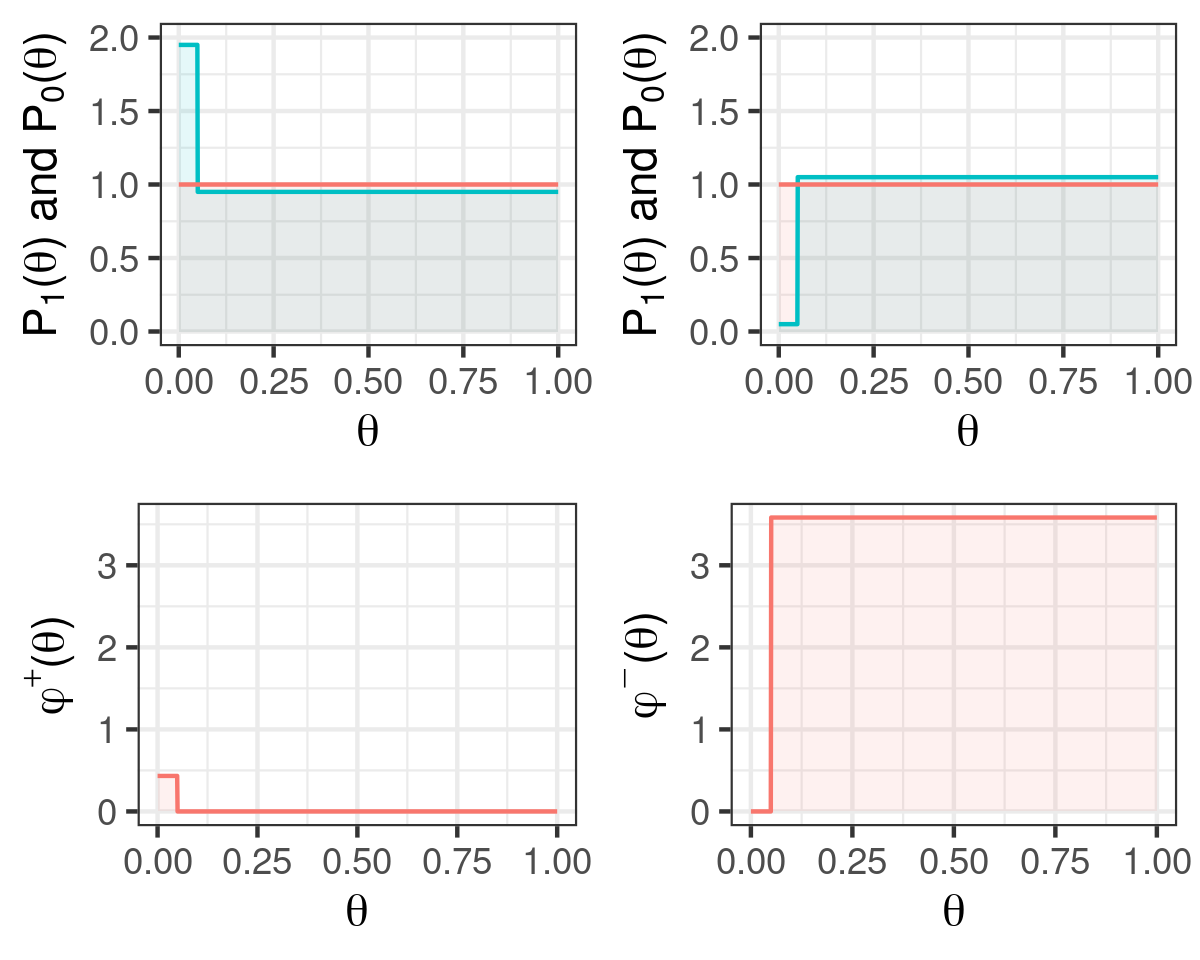
\includegraphics[width=0.980\linewidth,height=0.784\linewidth]{figure/positive_pert-1} 

}

\caption{A plot of the perturbations from \exref{positive_pert_large} with $p=2$ and $\epsilon=0.05$.  Positive $\phi$ can only add mass, so to remove a small amount of mass requires adding mass everywhere else and re-normalizing, resulting in a large perturbation according to $\norm{\cdot}_p$.}\label{fig:positive_pert}
\end{figure}


\end{knitrout}
}


\newcommand{\FunctionPathsFig}{

\begin{knitrout}
\definecolor{shadecolor}{rgb}{0.969, 0.969, 0.969}\color{fgcolor}\begin{figure}[!h]

{\centering 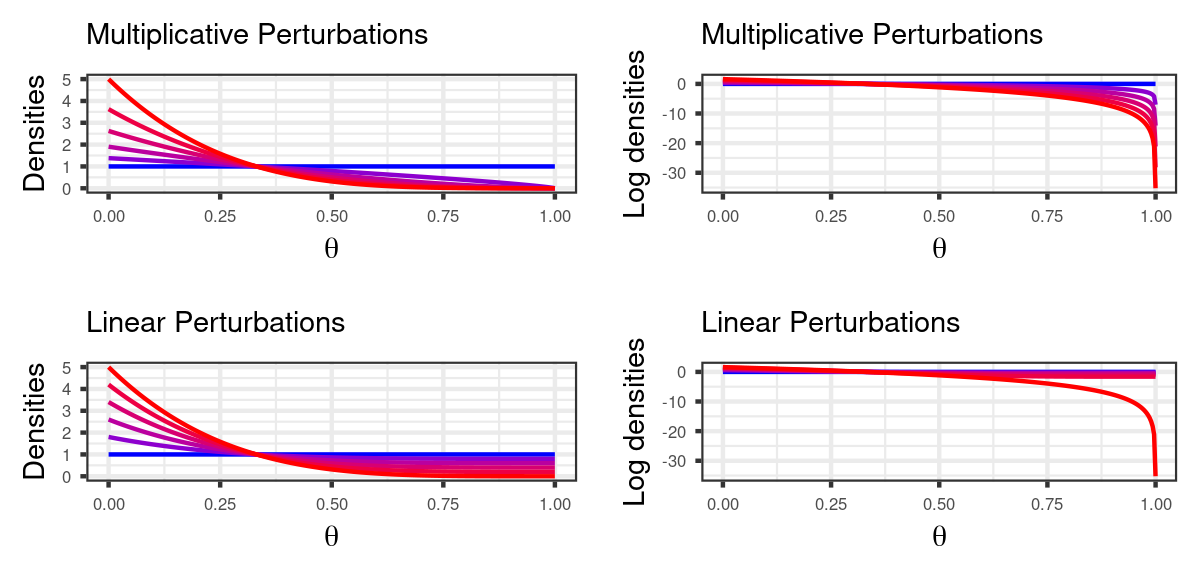
\includegraphics[width=0.980\linewidth,height=0.470\linewidth]{figure/path-1} 

}

\caption[Multiplicative and linear mixture paths between two densities]{Multiplicative and linear mixture paths between two densities.}\label{fig:path}
\end{figure}


\end{knitrout}
}


\newcommand{\FunctionPathsMultFig}{

\begin{knitrout}
\definecolor{shadecolor}{rgb}{0.969, 0.969, 0.969}\color{fgcolor}\begin{figure}[!h]

{\centering 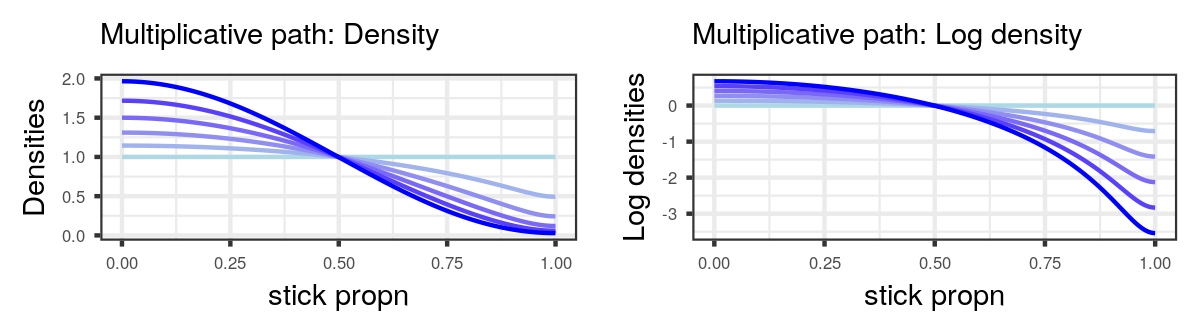
\includegraphics[width=0.980\linewidth,height=0.274\linewidth]{figure/mult_path-1} 

}

\caption[Multiplicative mixture paths between two densities]{Multiplicative mixture paths between two densities.}\label{fig:mult_path}
\end{figure}


\end{knitrout}
}


\newcommand{\FunctionPathsLinFig}{

\begin{knitrout}
\definecolor{shadecolor}{rgb}{0.969, 0.969, 0.969}\color{fgcolor}\begin{figure}[!h]

{\centering 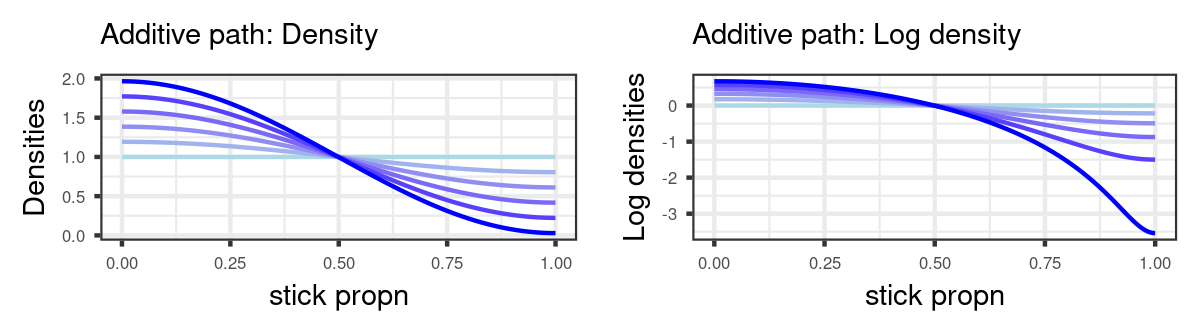
\includegraphics[width=0.980\linewidth,height=0.274\linewidth]{figure/lin_path-1} 

}

\caption[Linear mixture paths between two densities]{Linear mixture paths between two densities.}\label{fig:lin_path}
\end{figure}


\end{knitrout}
}


\newcommand{\FunctionBallFig}{

\begin{knitrout}
\definecolor{shadecolor}{rgb}{0.969, 0.969, 0.969}\color{fgcolor}\begin{figure}[!h]

{\centering 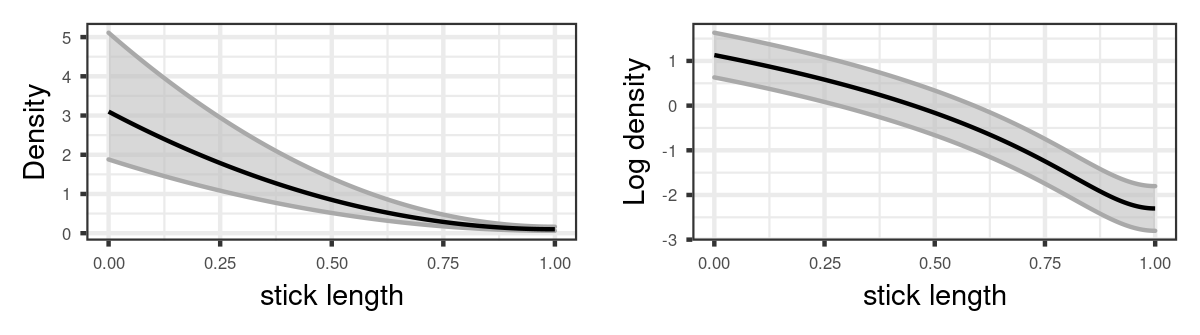
\includegraphics[width=0.980\linewidth,height=0.274\linewidth]{figure/func_ball-1} 

}

\caption[An multiplicative ball $\ball_\phi(\delta)$]{An multiplicative ball $\ball_\phi(\delta)$.}\label{fig:func_ball}
\end{figure}


\end{knitrout}
}



\newcommand{\FunctionDistFig}{

\begin{knitrout}
\definecolor{shadecolor}{rgb}{0.969, 0.969, 0.969}\color{fgcolor}\begin{kframe}


{\ttfamily\noindent\bfseries\color{errorcolor}{\#\# Error in FUN(X[[i]], ...): object 'p' not found}}\end{kframe}\begin{figure}[!h]

{\centering 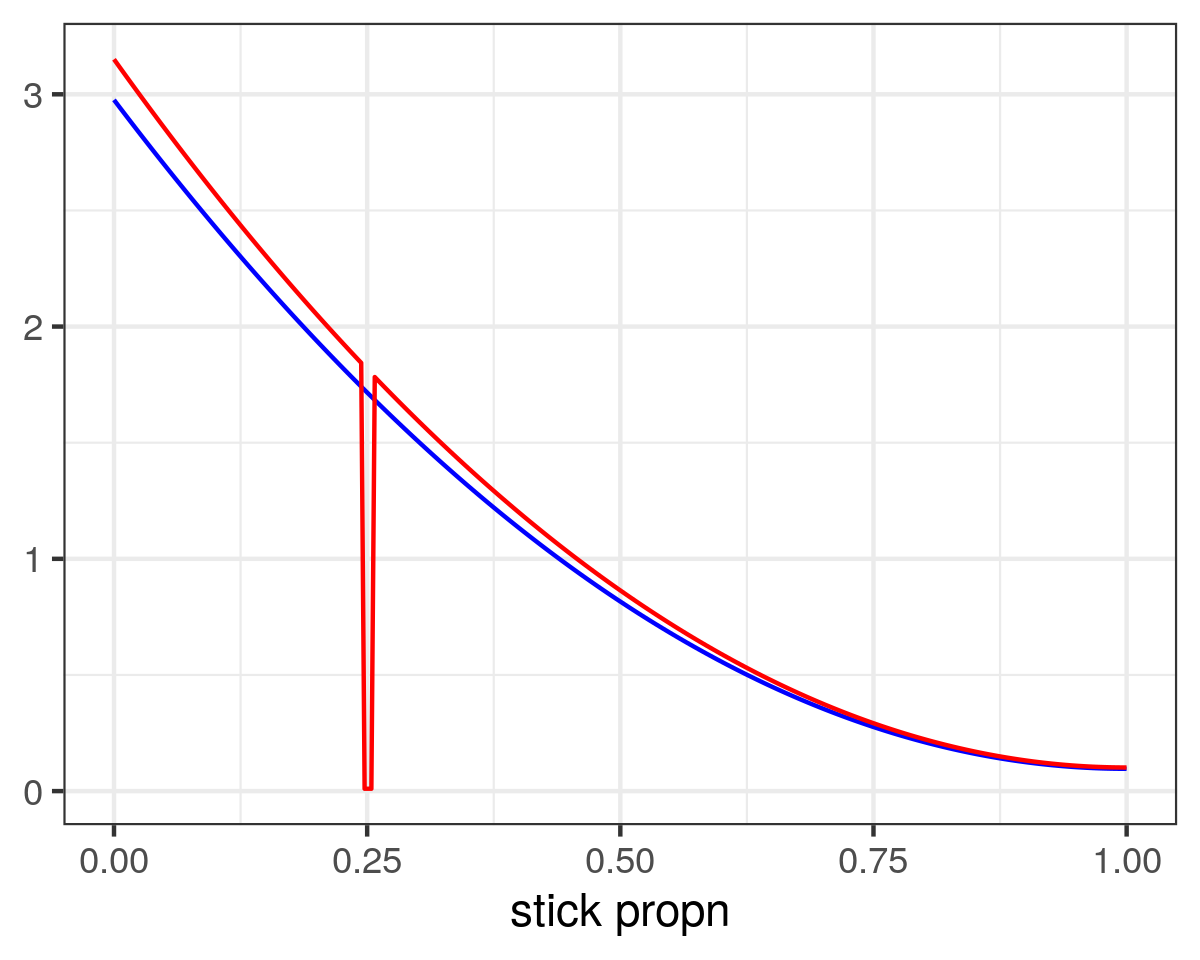
\includegraphics[width=0.980\linewidth,height=0.470\linewidth]{figure/func_dist-1} 

}

\caption[Two densities which are distant according to KL divergence and $\norminf{\cdot}$ but close according to $\norm{\cdot}_p$ for $p \in [1, \infty)$]{Two densities which are distant according to KL divergence and $\norminf{\cdot}$ but close according to $\norm{\cdot}_p$ for $p \in [1, \infty)$.}\label{fig:func_dist}
\end{figure}


\end{knitrout}
}
